\chapter{Analýza a rešerše}\label{analyza}

\section{Architektura apliakce}\label{analyza-architektura}

Jako doporučenou architekturu aplikací pro platformu iOS (konkrétně iPhone a iPad) uvádí Apple Model-View-Controller (zkráceně MVC).
Přestože je MVC pro vývoj aplikací nejpopulárnější, rozhodl jsem před začátkem implementace prozkoumat i jiné existující architektury.
Z alternativních architektur jsem nakonec zvolil Model-View-ViweModel, kterou porovnám s dopručeným MVC.
V závislosti na výsledku porovnání zvolím ideální architekturu pro svou aplikaci.

\subsection{MVC: Model-View-Controller}\label{analyza-mvc}
Tato architektura rozděluje aplikaci do tří vrstev: Model, View a Controller.

\subsubsection{Popis architektury}

\begin{description}
  \item[Model] reprezentuje perzistentní objekty, které aplikace využívá pro vnitřní logiku a prezentaci dat uživateli.
  Každý modelový objekt může být v relaci s libovolným počtem jiných modelových objektů.
  Tato vrstva je často reprezentována databází, příkladem mohou být databáze CoreData, Realm nebo SQLite.

  \item[View] je datový objekt viditelný uživatelem. View obsahuje logiku pro vykreslení a interakci s uživatelem.
  Přestože se View standardně používá pro zobrazení modelových objektů nebo jejich úpravu, jsou od sebe tyto vrstvy striktně odstíněny.
  Na platformě iOS tuto vrstvu reprezentuje framework UIKit vytvořený Applem.

  \item[Controller] je aplikační vrstva, která na základě vstupů z View aktualizuje a mění Model nebo překresluje View v případě, že zobrazovaná data už nejsou aktuální.
  Jedním z úkolů Controlleru je striktně zamezit přímé interakci mezi View a Modelem.
  Toto oddělení je zavedeno proto, aby View nemuselo znát konkrétní strukturu Modelu a aby Model nemusel obsahovat logiku formátování dat (cena, čas, ...) pro vykreslení.
  Dále se stará o navigaci mezi obrazovkami, síťování a interakci s uživatelem.
  Při rozdělení do obrazovek platí pravidlo, že jeden controller obsluhuje jedno nebo více View.
  Ke korektnímu vykreslení View využívá libovoné množství modelových objektů.
  O jednu obrazovku se typicky stará právě jeden Controller, je ale možné jich použít více.
\end{description}

\begin{figure}\centering
	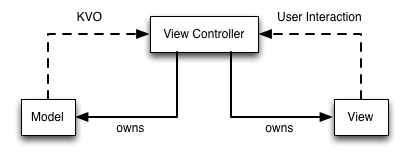
\includegraphics[width=0.5\textwidth]{assets/mvc-architecture.png}
	\caption[Architektura MVC]{Architektura MVC}\label{fig:architektura-mvc}
\end{figure}

Z tohoto shrnutí vyplývá, že Controller je velmi blízce spjat s View. Toto propojení reprezentuje obrázek \ref{fig:massive-mvc}.

\begin{figure}\centering
	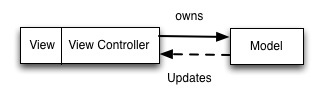
\includegraphics[width=0.5\textwidth]{assets/mvc-massive-view-controller.png}
	\caption[Role Controlleru v MVC]{Controller spjatý s View}\label{fig:massive-mvc}
\end{figure}

\subsubsection{Modelový příklad použití}

Pro možné porovnání architektury jsem připravil scénář stažení libovolných dat na základě požadavku uživatele.
V MVC by se architektura chovala takto:

\begin{itemize}
  \item Uživatel v aplikaci klikne na tlačítko \uv{Stáhnout data}.
  \item Tuto interakci odchytí view a upozorní controller.
  \item Controller na základě upozornění stáhne data a předá je modelu k uložení.
  \item Model ukládá data a notifikuje controller o změně.
  \item Controller aktualizuje view.
  \item Nastane-li během stahování chyba, controller vytváří nové view a chybu prezentuje uživateli.
\end{itemize}

\subsubsection{Shrnutí}

Shrneme-li vlastnosti vrstev, jejich klíčové role jsou:

\begin{itemize}
  \item Model udává, jakým způsobem jsou data uložena,
  \item View se stará o správné vykreslení předformátovaných dat,
  \item Controller se stará o ostatní logiku.
\end{itemize}

Pro zmíněné notifikace nabízí Apple řešení pomocí Delegate pattern.
Controller musí naimplementovat specifické rozhraní, čímž se stane delegátem.
Jako delegát se pak může zaregistrovat na notifikace obejktů, jejichž rozhraní implementoval.

MVC je v době psaní této práce nejpoužívanější architekturou a to především díky své jednoduchosti.
Při tvorbě větších aplikací ale nemusí být vhodné.
Controller se při nestandradním grafickém návrhu může stát velmi složitým, což výrazně snižuje jeho čitelnost a testovatelnost.
Z tohoto důvodu se MVC často přezdívá \uv{Massive View Controller}.
Díky přímému napojení controlleru na View se při testování chování Controlleru (behavioral testing) musí využít simulátoru mobilního operačního systému a aplikaci v něm automaticky \uv{proklikat}.
To zvyšuje časovou náročnost testování, dokonce v některých případech znemožňuje testování úplně (controlleru nezle podvrhnout mock objekty).
Tento problém se snaží řešit architektura MVVM od společnosti Microsoft.

\subsection{MVVM: Model-View-ViewModel}\label{analyza-mvvm}

Z důvodu nárustu nároků na mobilní aplikace se v posledních letech rozmáhá architektura MVVM.
Tato architektura vychází ze zmíněného MVC a jejím základním úkolem je zjednodušit Controller.

\subsubsection{Popis architektury} \label{architektura-mvvm-popis}

Za účelem zjednodušení Controlleru se ke stávajícím třem vrstvám přidává View Model, který se stará o přípravu dat z Modelu pro zobrazení a také o perzistenci změn.

\begin{description}
  \item[View Model] je objekt vlastněný controllerem za pomoci kompozice.
  Pro Controller připravuje naformátované výstupy a poskytuje mu rozhraní pro vstupy.
  Výstupem se rozumí veškerá data, která jsou potřebná pro sestavení View.
  To může být např. datum ve specifickém formátu, cena včetně měny nebo informace o tom, kolik řádků bude obsahovat tabulka na obrazovce.
  Oproti MVC tedy perzistentní data nejsou viditelná Controlleru, ale pouze View Modelu.
  Ten je nejdříve připraví pro zobrazení.
  Vstupem může být libovolná interakce uživatele:
  změna textu v textovém poli, stisknutí tlačítka, ale i fyzický pohyb telefonem (otočení obrazovky).
  Na základě vstupů spouští View Model svou vnitřní logiku a generuje výstupy.
\end{description}

Zodpovědnost Controlleru se zavedením View Modelu dramaticky snižuje.
V ideálním případě je Controller zodpovědný pouze za správné sestavení View a napojení zfromátovaných výstupů na něj.
Dále pak za odchycení uživatelských interakcí a jejich propagaci do View Modelu.
Toto chování zachycuje obrázek \ref{architektura-mvvm}.

\begin{figure}\centering
	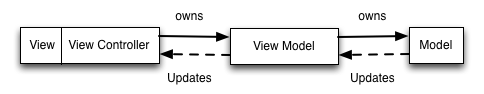
\includegraphics[width=0.5\textwidth]{assets/mvvm-architecture.png}
	\caption[Architektura MVVM]{Architektura MVVM}\label{architektura-mvvm}
\end{figure}

\subsubsection{Modelový příklad použití} \label{architektura-mvvm-priklad}

Pro porovnání architektury s MVC lze opět využít scénář pro stažení dat. Pro tento scénář by se architektura MVVM chovala následovně:
\begin{itemize}
  \item Controller napojuje výstupy view modelu na view a vytváří pravidla pro převod uživatelské interakce na vstupy view modelu.
  \item Uživatel v aplikaci klikne na tlačítko "Stáhnout data".
  \item View upozorňuje controller na interakci uživatele, ten automaticky vytváří vstup pro view model.
  \item View model na základě vstupu stahuje data a předává je modelu.
  \item Model po uložení notifikuje view model, ten vytváří výstup pro controller, který nechává překreslit view.
  \item V případě chyby vytvoří view model chybový výstup, ten se pomocí controlleru propaguje do view.
\end{itemize}

\subsubsection{Shrnutí} \label{architektura-mvvm-shrnuti}

Vrstvy mají následující klíčové vlastnosti:
\begin{itemize}
  \item Model definuje jakým způsobem jsou data uložena a při změně notifikuje View Model,
  \item View vykresluje na obrazovku naformátované výstupy a upozorňuje controller při interakci uživatele,
  \item Controller sestavuje hierarchii view, napojuje zformátované výstupy view modelu na view a z uživatelské interakce vytváří vstupy pro view model,
  \item View model načítá data modelu, na základě vstupů z controlleru nebo změny modelu generuje výstupy pro controller.
\end{itemize}

Oproti MVC je na tomto příkladu vidět snížení zodpovědnosti controlleru. Tato zodpovědnost se přesunula do View Modelu.
Na první pohled nemusí být tato změna opodstatněná, protože logika aplikace nezmizela, jen se přesunula.
Právě to ale umožnilo (nebo minimálně zjednodušilo) způsob, jakým lze logiku testovat.
View Model generuje výstupy na základě vstupů, v testech tedy lze uživatelskou interakci podvrhnout a testovat pouze výstupy (není potřeba vytvářet View ani Controller).
Dodatečně lze otestovat i uživatelské rozhraní.
Protože logika aplikace je otestována pomocí testů View Modelu, uživatelské rozhraní už stačí otestovat např. shodou View s referenčním obrázkem.

Při pohledu na notifikace je vidět, že přibyl typ, který nebyl v MVC potřeba.
Jedná se o notifikace směrem z View Modelu ke Controlleru (View Model nemá referenci na Controller, nemůže ho notifikovat přímo).
Některé výstupy view modelu je tedy potřeba sledovat v čase a na jejich změny reagovat.
Toto lze vyřešit pomocí KVO, které nabízí Apple v základu.
KVO umožňuje objektu zaregistrovat se na notifikace o změně stavu nějakého libovolného objektu.
V případě Controlleru by se registroval na změny stavu výstupů View Modelu.
Kdykoliv by se výstup změnil, Controller by dostal notifikaci.
Tento přístup ale není běžný pro použití s jazykem Swift.
Tento postup navíc neřeší synchronizaci vláken, z tohoto důvodu by mohlo docházet k nekonzistenci dat či neočekávanému chování.
Místo KVO se nyní standardně používají reaktivní rozšíření, které popisuji v následujících kapitolách.

Přestože mnou implementovaná aplikace není v ohledu na uživatelské scénáře nijak složitá, obsahuje mnoho obrazovek.
Obrazovky jsou vysoce interaktivní a více se k jejich implementaci hodí reaktivní přístup.
Z tohoto důvodu jsem jako architekturu vybral MVVM s použitím reaktivních rozšíření místo standardního MVC.

\section{Synchronizace vláken aplikace} \label{analyza-synchronizace-vlaken}

Mobilní aplikace se svou povahou značně liší od běžných webových nebo desktopových aplikací.
Oproti zmíněným jsou často mnohem interaktivnější, tedy ovládané nejen běžnými vstupy, ale i vlastnostmi zařízení (GPS poloha, orientace zařízení, dostupnost periferií).
Aby tyto vstupy nekazily uživatelský zážitek, jsou v systému implementovány asynchronně.

Jako příklad lze vzít získávání polohy z družic.
To provádí telefon na vlákně v pozadí.
Tím je zaručené, že hlavní vlákno aplikace (které se mimo jiné stará o vykreslování) není blokované a s aplikací lze bez problému intereagovat.
Jakmile jsou dostupné informace o poloze, aplikace zažádá systém o prostředky na hlavním vlákně a získanou polohu prezentuje uživateli.

Tento přístup je v SDK poskytovaným Applem velmi obvyklý a využívá ho mnoho standardních knihoven.
Ne vždy je ale běžné, aby výsledek byl prezentovaný na hlavním vlákně.
Takový princip je využit u síťových požadavků.

Síťový požadavek se vykonává na vlákně v pozadí a na stejném vlákně je zpracována i odpověď ze vzdáleného serveru.
Je-li potřeba odpověď zpracovat na hlavním vlákně, musí vývojář explicitně čas na hlavním vlákně vyžádat pomocí Grand Central Dispatch či vlákna synchronizovat jiným spůsobem.
Od verze systému iOS 9 je navíc nemožné udělat síťový požadavek synchronně (blokovat vlákno, které požadavek vytvořilo až do konce zpracování) \cite{apple-whats-new-in-ios}.

Otázkou tedy zůstává jak správně synchronizovat všechny vlákna, která potřebují zpracovat data na hlavním vlákně.

Při analýze tohoto problému jsem se zaměřil na tři možná řešení.
První dvě jsou implementovány přímo v dodávaném SDK, třetí možnost je knihovna od společnosti GitHub.

\subsection{Grand Central Dispatch}

Grand Central Dispatch (zkráceně GCD) je technologie vyvinutá společností Apple přinášející optimalizovanou podporu pro aplikace fungující na vícejádrových procesorech.
GCD je implementována nad standardními systémovými vlákny, vývojáři ale nabízí mnohem jednoduší rozhranní.

Pro zjednodušení je využit princip front (z angl. queue), které jsou reprenzentovány třídou \textit{DispatchQueue}.
DispatchQueue je implementována jako \textit{thread-safe}, je tedy možné k nim přistupovat ve stejný okamžik z několik vláken najednou \cite{apple-concurrency-programming-guide}.
Do této fronty je možné vkládat jednotky práce, GCD se postará o to aby byly spuštěny na ve správném pořadí.
V závislosti na konfiguraci je pak umožňuje jednotlivé úkoly spouštět synchronně nebo asynchronně.

V základu je dostupná \textit{main} fronta, která je synchronní a umožňuje vykonat práci na hlavním vlákně.
Pro synchronizaci vláken stačí požadované jednotky práce přidávat do správných front  \ref{code:create-dispatch-queue}.

Je-li potřeba vytvořit vlastní frontu (z důvodu uvolnění času na hlavním vlákně), stačí specifikovat název fronty a její prioritu.
Vytvoření nové fronty běžící v pozadí je vidět v ukázce \ref{code:create-dispatch-queue}.

\swiftcode{code:create-dispatch-queue}{GCD: Vytvoření vlastní fronty}{assets/code/create-dispatch-queue.swift}

Přidání do libovolné fronty..

\subsubsection{Quality of Service}

Pro možnost rozlišení priorit front využívá Apple Quality of Service (zkráceně QoS).
Díky QoS je možné určit, jakou prioritu bude mít danná fronta při rozdělování vláken.
V současné době existují čtyři QoS priority \ref{apple-prioritize-work-with-qos}:

\begin{description}
  \item[User-interactive] Práce, se kterou uživatel přímo interaguje.
  Tato fronta má nejvyšší prioritu, nejčastěji se v ní provádí překreslování uživatelského rozhranní či animace.
  Jednotlivé úkoly z fronty jsou vykonané ihned.
  \item[User-initiated] Práce, kterou zadal uživatel a vyžaduje okamžitý výsledek.
  Nejčastěji se stará o akce, které nastanou po interakci s některým z ovládacích prvků (např. tlačítko).
  \item[Utility] Práce, která vyžaduje více času pro své dokončení.
  Typicky se jedná o síťové požadavky nebo načítání dat.
  \item[Background] Práce s nízkou prioritou, kterou si nevyžádal uživatel.
  Využívá se zejména pro dávkové mazání souborů, synchronizaci nebo indexování databáze.
\end{description}

Při vytváření front je důležité správně volit prioritu.
Budou-li všechny fronty využívat jednu prioritu, může se stát, že systémová vlákna nebudou správně využita.
To by vedlo ke snížení výkonu aplikace a špatné uživatelské zkušenosti.

Přestože GCD je velmi zajímavá abstrakce nad standardními vlákny, jedná se stále o nízkoúrovňové API.
Mezi jednotkami práce nelze vyvářet závislosti či je řetězit.
Tuto možnost ale nábízí \textit{Foundation} framework pomocí \textit{NSOperationQueue}.

\subsection{NSOperationQueue a NSOperation}

NSOperationQueue a NSOperation je abstrakce nad metodou GCD zmíněnou víše.
Toto API je od verze systému iOS 4 implementováno právě pomocí GCD, nabízí ale nové možnosti přístupu k prováděným jednotkám práce.
Hlavním rozdílem oproti GCD je vyloučení pojmu \textit{vlákno}.
Jednotky práce nejsou nadále reprezentovány pomocí \textit{first class funkcí}, ale nově pomocí instancí tříd \textit{NSOperation} o jejichž správu se stará \textit{NSOperationQueue}. \cite{cocoacasts-nsoperation-vs-gcd}

\subsubsection{NSOperation}

Pro reprezentaci jednotek práce se standardní funkce v GCD nejevily jako dostatečné.
S představením NSOperationQueue, je ale nově možné nad opakovanými jednotkami abstrakci pomocí tříd.
Toho lze docílit pomocí vytváření vlastních tříd dědících od NSOperation.

NSOperation představuje samostatnou jednotku práce (operaci).
Jedná se o abstraktní třídu zajišťující \textit{thread-safe} přístup ke správě stavu, priority a závislostí.

Jako úkol lze chápat například jednotlivé síťové požadavdy, zpracování vstupů a uživatele a jejich perzistence nebo komplexní výpočty.
Úkolem je možné označit ale i libovolnou strukturovanou jednotku práce, u které je potřeba udržovat stav nebo zpracovat její datový výstup.

Oproti CGD má objektový přístup výhodu nejen v přehlednější strukturování, ale i v možnosti vytváření závislostí a správě stavu \cite{apple-operation-queues}.

\begin{description}
  \item[Závislosti] definují, jaké další operace musí být vykonány před tím, než bude daná operace spuštěna.
  Přidat lze libovolný počet dalších operací, tím lze dosáhnout komplexního procesu za pomoci skládání menších bloků.
  Jako příklad lze uvést síťovou komunikaci, kde každý požadavek závisí na ověření dostupnosti internetu (první operace) a na patřičném ověření uživatele (druhá operace).
  Ke každému požadavku následně stačí přiřadit tyto dvě operace jako závislost, tím je zaručené že požadavek se pošle jen když je dostupné připojení k internetu a zároveň je uživatel ověřený.
  \item[Správa stavu] umožňuje operaci pozastavit, spustit znovu nebo zrušit.
  Oproti GCD, kde úkol, který se začal zpracovávat už nebylo možné zastavit, lze například do ovládání operací zapojit uživatele.
\end{description}

\subsubsection{NSOperationQueue}

Obdobně jako GCD, je i zde potřeba určit kde a kdy se bude práce vykonávat.
Pro tento účel slouží fronta NSOperationQueue.
Tato fronta je implementována jako prioritní.
Tedy v momentě kdy je vložena operace s vyšší prioritou, bude vykonána dříve než stávající operace s nízkou prioritou (pokud to její závislosti dovolí).
Z tohoto odůvodu není zaručeno kdy se jednotlivé operace spustí.

Základní vytvoření operace a vložení do fronty je vidět na ukázce \ref{code:operation-queue-demonstration}.

\swiftcode{code:operation-queue-demonstration}{NSOperationQueue: Vytvoření fronty s operacemi}{assets/code/operation-queue-demonstration.swift}

\subsubsection{Prioritizace úkolů}

Z důvodu potřeby prioritizace některých úloh je možné jedntlivým operacím nastavit prioritu.
V takovém případě se vždy jako první vykonají operace s vyšší prioritou, následně se přistupuje k těm s nižším.

\subsubsection{Quality of Service}

Jednou z nejsilněších stránek NSOperationQueue je abstrakce front nad vlákny (tedy celého GCD).
V nastavení fronty lze zvolit stejně jako u GCD výchozí QoS.
Všechny operace pak budou vyžívat právě tuto prioritu.
Oproti GCD má však NSOperationQueue výhodu, že nepracuje pouze s jednou frontou.

To dává vývojáři možnost definovat QoS pro každou operaci zvlášť a to bez nutnosti vytvořát více front.
V závisloti na této vlastnosti je dále možné definovat, kolik operací může být \textit{maximálně} spuštěno v jeden okamžik.
